\chapter{User Manual}

\section{Introduction}

In this manual I will go through the correct way to install and utilise the program to its best abilities. The user will require a computer which meets certain specifications and a CD-ROM holding a zip file of the application. The intended audience for the system was the director of Perfect Publishers Ltd.

\section{Installation}

\subsection{Prerequisite Installation}

As the system has been compiled to a windows executable, the system does not require any programs to be installed on the computer which it is to be used on apart from the system itself. The program was intended to run on Windows 7/8, as these were the operating systems that it was designed on, and the operating system that the client owns.

The following is required for the system to reach its full capabilities:

\begin{itemize}
    \item A Keyboard for user inputs
    \item A Mouse for user inputs
    \item A Hard Disk Drive for storage
    \item A Visual Display Unit for outputs generated by the system
    \item Connection the the internet if the user needs an email sent to their email when they've forgotten their password
    \item At least 512 megabytes of main memory to carry out processing
\end{itemize}


\subsection{System Installation}

The user requires the CD-R that has the necessary files on for installation. 


After inserting the CD-R, the user will need to open 'My Computer'.

\begin{figure}[H]
    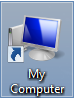
\includegraphics[width=\textwidth]{./Manual/Installation/MyComputer.png}
\end{figure}

The user will then need to right click the CD-R, and click open.

\begin{figure}[H]
    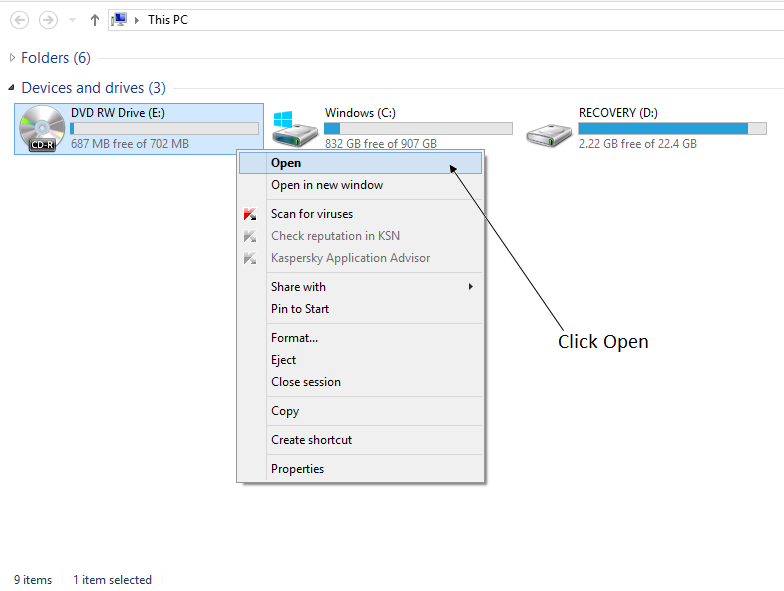
\includegraphics[width=\textwidth]{./Manual/Installation/OpenCDR.png}
\end{figure}

Then right click on the installation file, and click 'Install'.

\begin{figure}[H]
    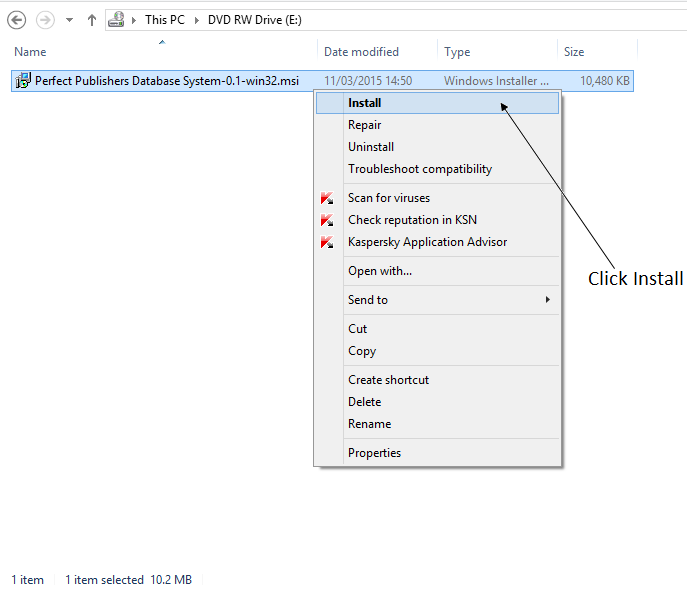
\includegraphics[width=\textwidth]{./Manual/Installation/Install.png}
\end{figure}

The Windows installer will the commence installing. The user is required to select a destination to be installed at, with the default directory given.

\begin{figure}[H]
    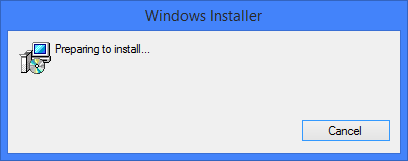
\includegraphics[width=\textwidth]{./Manual/Installation/PrepareInstall.png}
\end{figure}

\begin{figure}[H]
    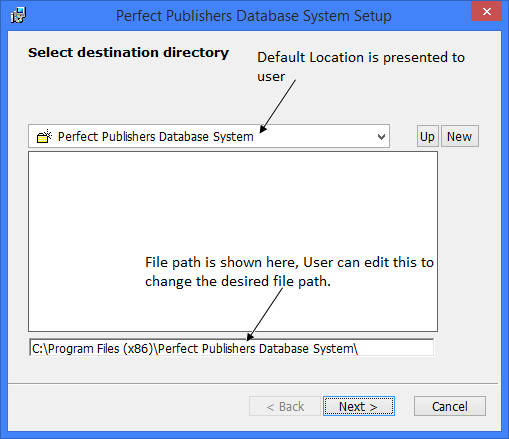
\includegraphics[width=\textwidth]{./Manual/Installation/Setup.png}
\end{figure}

\begin{figure}[H]
    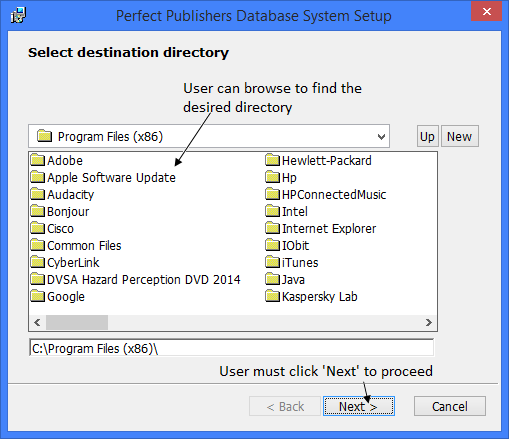
\includegraphics[width=\textwidth]{./Manual/Installation/Setup2.png}
\end{figure}

The Installer initialises the screen for installation.

\begin{figure}[H]
    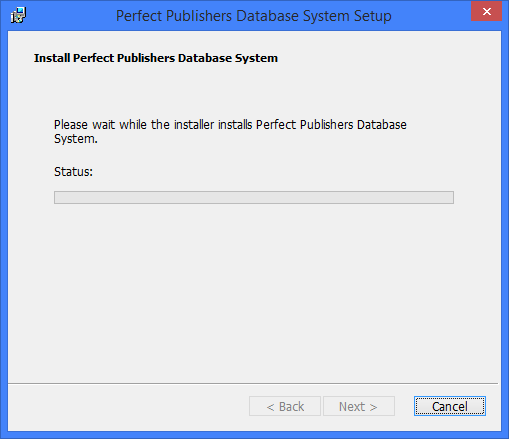
\includegraphics[width=\textwidth]{./Manual/Installation/PleaseWaitScreen.png}
\end{figure}

The user must grant the installer permission to complete installation. To do so, click 'Yes' when the prompt opens.

\begin{figure}[H]
    
\includegraphics[width=\textwidth]{./Manual/Installation/Permission.png}
    \caption{Prompt for permission}
\end{figure}

Once the user has granted the installer permission, the installation is completed.

\begin{figure}[H]
    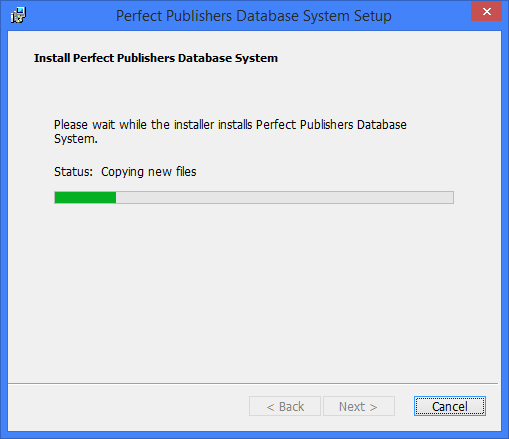
\includegraphics[width=\textwidth]{./Manual/Installation/Installing.png}
\end{figure}

\begin{figure}[H]
    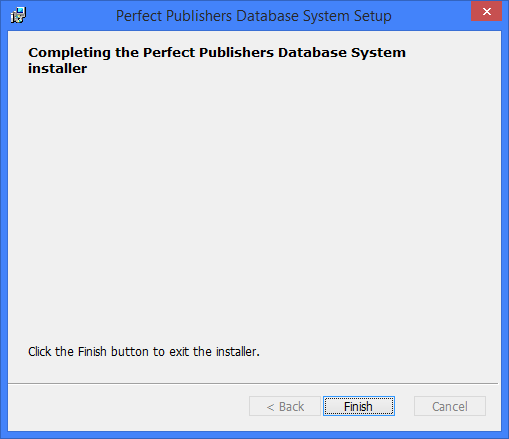
\includegraphics[width=\textwidth]{./Manual/Installation/Installed.png}
\end{figure}


\subsection{Running the System}

In order to run the system, the user could navigate to the path of installation, or the user could create a shortcut to run quickly.

To create a shortcut, the user must do the following:

\begin{figure}[H]
    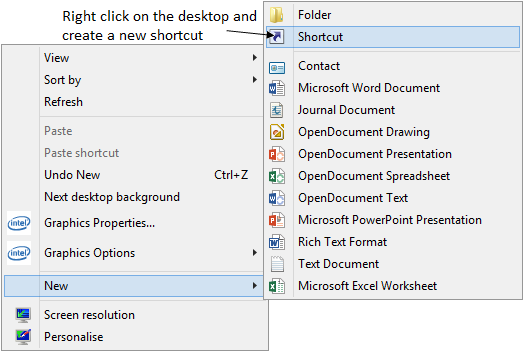
\includegraphics[width=\textwidth]{./Manual/Installation/Shortcut.png}
\end{figure}

\begin{figure}[H]
    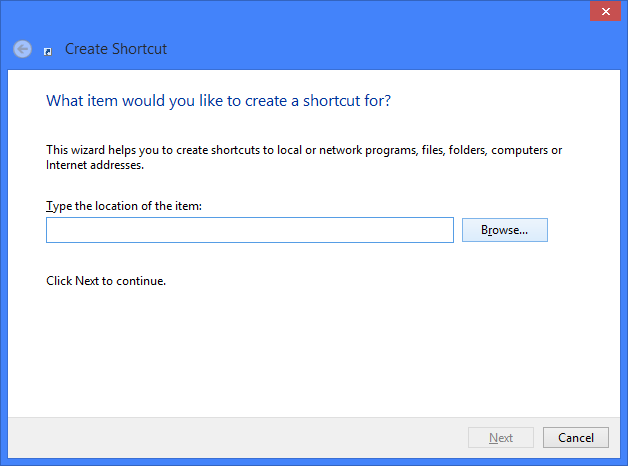
\includegraphics[width=\textwidth]{./Manual/Installation/CreateShortcut.png}
\end{figure}

The user will be presented with the interface to type the file path of the system file. The user should click 'Browse...', where the user should browse to the correct file shown in Figure \ref{fig:BrowseFile}.

\begin{figure}[H]
    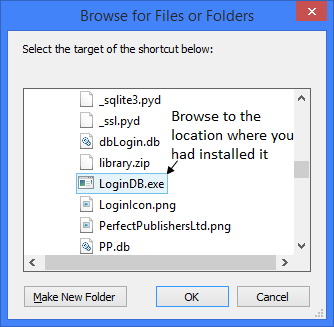
\includegraphics[width=\textwidth]{./Manual/Installation/BrowseFile.png}
    \label{fig:BrowseFile}
\end{figure}

Then the user is required to name the shortcut. Afterwards, the user needs to click finish to finish creating a shortcut that the program can be run from.

\begin{figure}[H]
    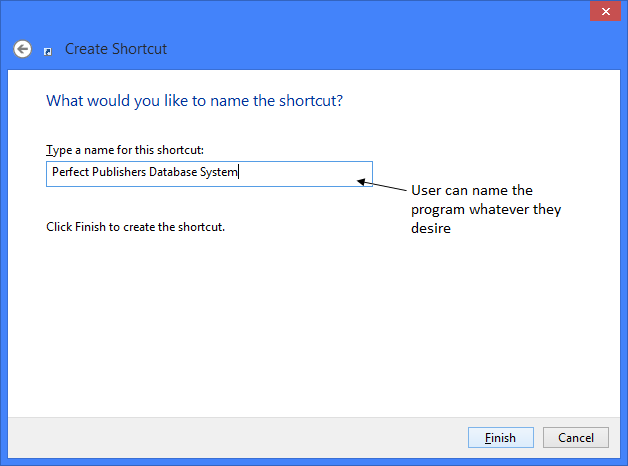
\includegraphics[width=\textwidth]{./Manual/Installation/NameShortcut.png}
    \label{fig:BrowseFile}
\end{figure}

\section{Tutorial}

\subsection{Introduction}

In this section I will go through the steps of using the system to its full capabilities, including adding, editing and deleting data in the database, conducting calculations to find costs and payment prices, and searching for data in the database. I will also cover the navigation of the program.

\subsection{Assumptions}

I expect that the user has at least a basic understanding of Windows 7/8. As my client is capable with using these operating systems, the tutorial should not be difficult to follow. Also, for functions in the system that have similar functionality, only one of these functions will be properly investigated in my tutorial. For example, I will cover how to search for a book, and in doing so, I can assume that the user will be able to conduct searches for Royalties/Invoices etc., because of the similar functionality.

\subsection{Tutorial Questions}

%include as many subsubsections as necessary for
 each question in your list
\subsubsection{Question 1}

\subsubsection{Question 2}

\subsection{Saving}

\subsection{Limitations}

\section{Error Recovery}

%include as many subsections as necessary for each error
\subsection{Error 1}

\subsection{Error 2}

\section{System Recovery}

\subsection{Backing-up Data}

In order to backup my program, the user will need a hard copy of the backup kept off site, perhaps through the usage of a USB drive. The user should backup the database file, as this is the only data that requires being backed up.

\subsection{Restoring Data}

In order to restore my program, the user will need to use the hardware used to back up the database.